%  report.tex
%
%  Version 0.1.0
%
%  Copyright 2015 Nick Hepler <nick.hepler@outlook.com>
%
%  This program is free software; you can redistribute it and/or modify
%  it under the terms of the GNU General Public License as published by
%  the Free Software Foundation; either version 2 of the License, or
%  (at your option) any later version.
%
%  This program is distributed in the hope that it will be useful,
%  but WITHOUT ANY WARRANTY; without even the implied warranty of
%  MERCHANTABILITY or FITNESS FOR A PARTICULAR PURPOSE.  See the
%  GNU General Public License for more details.
%
%  You should have received a copy of the GNU General Public License
%  along with this program; if not, write to the Free Software
%  Foundation, Inc., 51 Franklin Street, Fifth Floor, Boston,
%  MA 02110-1301, USA.
%

% Use a one-sided article template
\documentclass[oneside]{article}
% Decrease the margins a little
\usepackage{fullpage}

% Set up for including graphics
% We'll use png or pdf graphics
\usepackage[pdftex]{graphicx}
\DeclareGraphicsExtensions{.png,.pdf}

% Hyperref adds hyperlinks to the document automatically
% It's not much use yet, but it will be
\usepackage{hyperref}

% For including code into the document
\usepackage{verbatim}

% Tweak the default fonts a little
\renewcommand\rmdefault{bch}
\usepackage[small]{caption}
\usepackage[small]{titlesec}
\linespread{1.07} 

\title{Statistical Analysis of Household Types and Incomes}
\author{Nick Hepler}
\date{February 20, 2015}

\raggedbottom

\begin{document}
\maketitle 

\section{Project Summary}

This source data set contains a sample of actual responses to the American Community Survey Public Use Microdata Sample (PUMS) from residents in New York State. Each observation represents a response from a single housing unit and the sample data represents responses from approximately one percent of the United States population.

Utilizing this data set, a comparative analysis of household income was conducted based upon households with no parent present in which the household was headed by a grandparent or not headed by a grandparent.

\section{Methods}

The source data was obtained through the American Community Survey Public Use Microdata Sample (PUMS) furnished by the United States Census Bureau, American Community Survey Office. The original data can be found on the Census FTP Site.

The R programming language was employed to perform the statistical analysis to include measures of central tendency and dispersion. In order to compare the two data samples, the data was subset using the NPP variable in the source data which denotes if a household with no parent present is headed by a grandparent. Missing data in the FINCP variable denoting annual household income was ignored, but negative income was included in the calculations. Calculations were rounded to the nearest hundredth.

\section{Data Considerations}

The raw data set contains 92,810 observations. Of these observations, the NPP variable was missing in 18,659 observations. Based on the rationale for this report, these observations were excluded leaving 74,151 observations remaining.

Of the 74,151 observations remaining, 25,732 had a missing value for the FINCP variable leaving 48,419 observations available for analysis. Of these observations, 48,156 observations were for households not headed by a grandparent with no parent present and the 263 remaining observations were associated with households headed by a grandparent with no parent present.

\newpage
\section{Summary Statistics}
\subsection{Not Grandparent Headed Household}

Measuring the central tendency of the data for households not grandparent headed, we find the average (n = 48,156) annual household income reported was \$95,153.96. The median household income was \$70,000.00. The minimum reported income was \$-12,800.00 and the maximum reported income was \$1,503,600.00. The range of the dispersion for income is \$1,516,400.00.

Measuring the variability of the sample data for this population we find the interquartile range of household income was \$80,990.00. The standard deviation of household income was \$101,243.48.

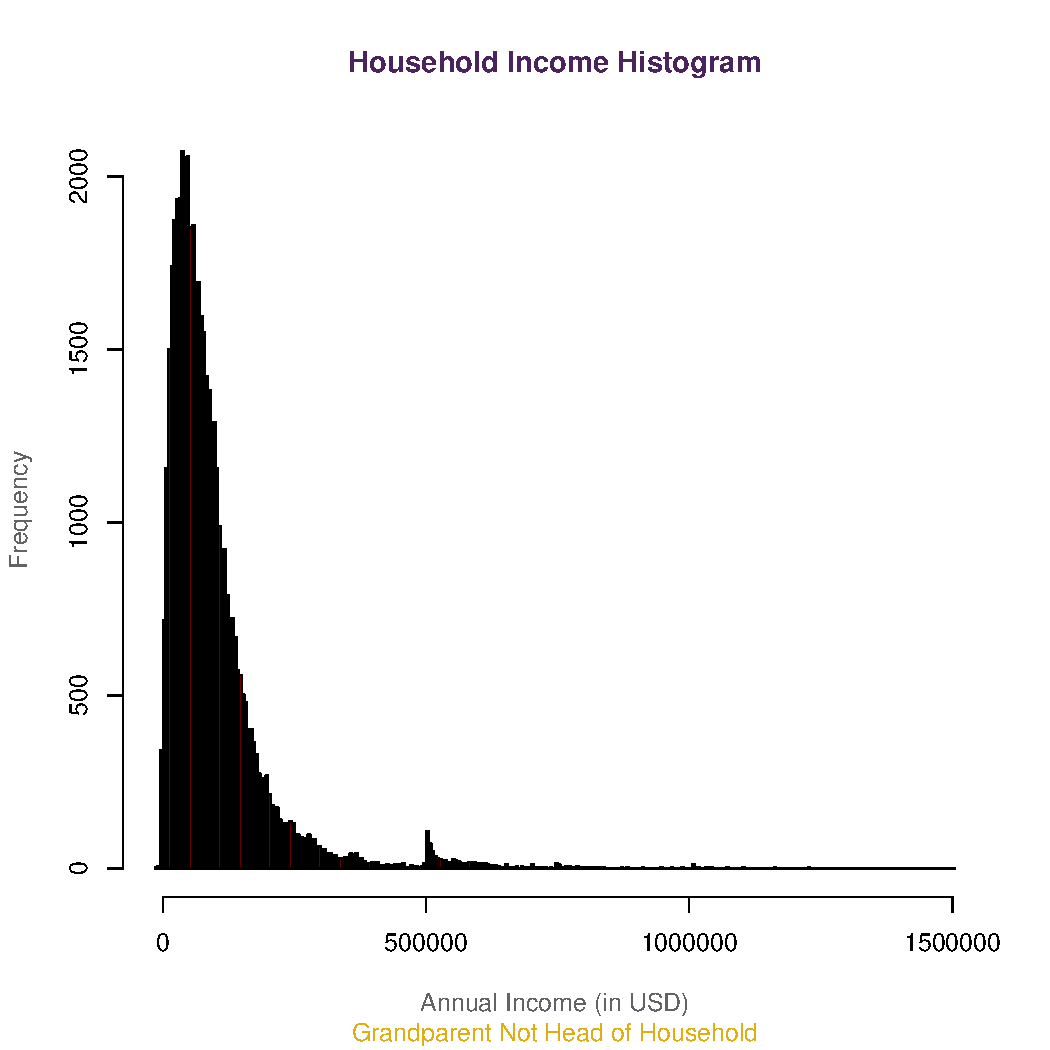
\includegraphics[width = .5\linewidth]{hist_nghh}
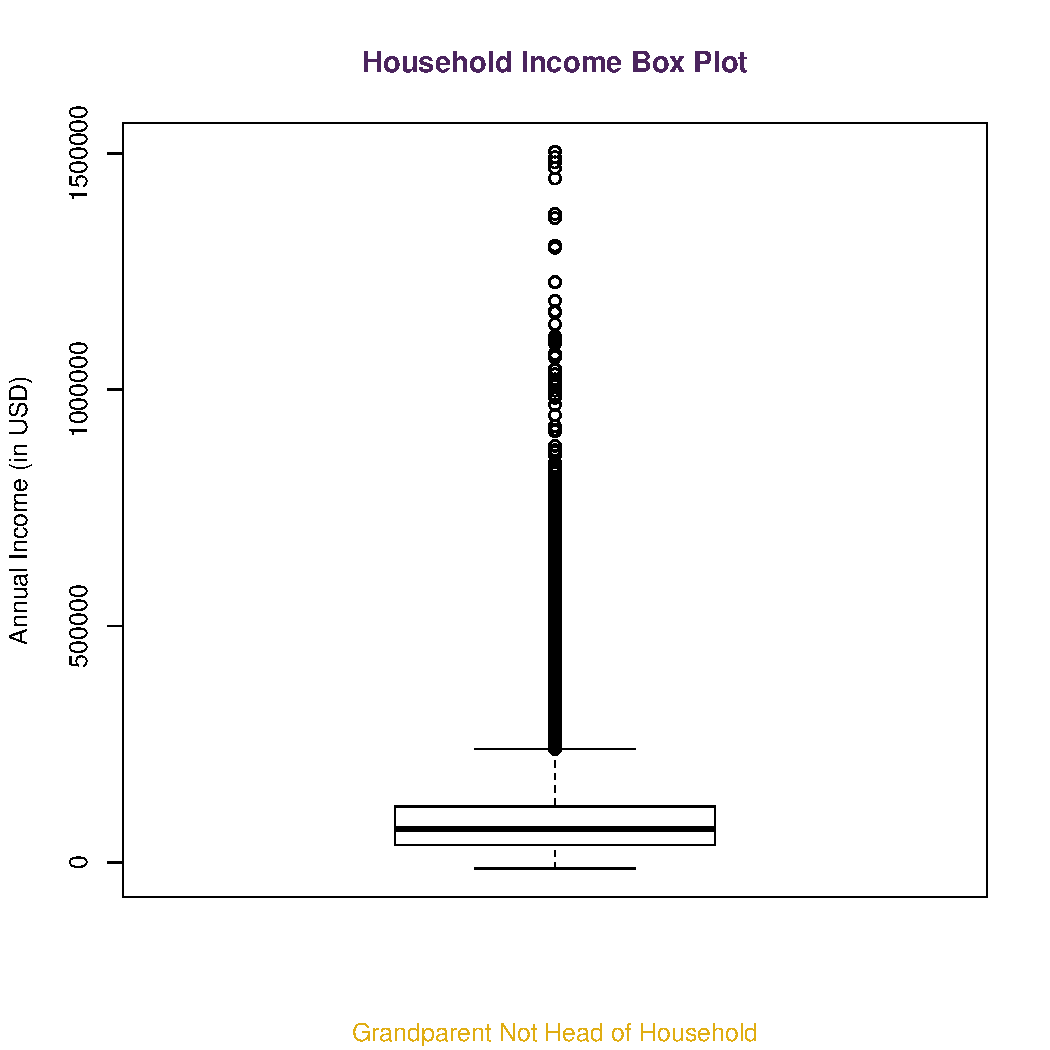
\includegraphics[width = .5\linewidth]{box_nghh}

\subsection{Grandparent Headed Household}

Measuring the central tendency of the data for grandparent headed households, we find the average (n = 263) annual household income reported was \$44,123.11. The median household income was \$30,400.00 The minimum reported income was \$0 and the maximum reported income was \$589,700.00.

Measuring the variability of the sample data for this population we find the interquartile range of household income was \$38,790.00. The standard deviation of household income was \$54,516.05.

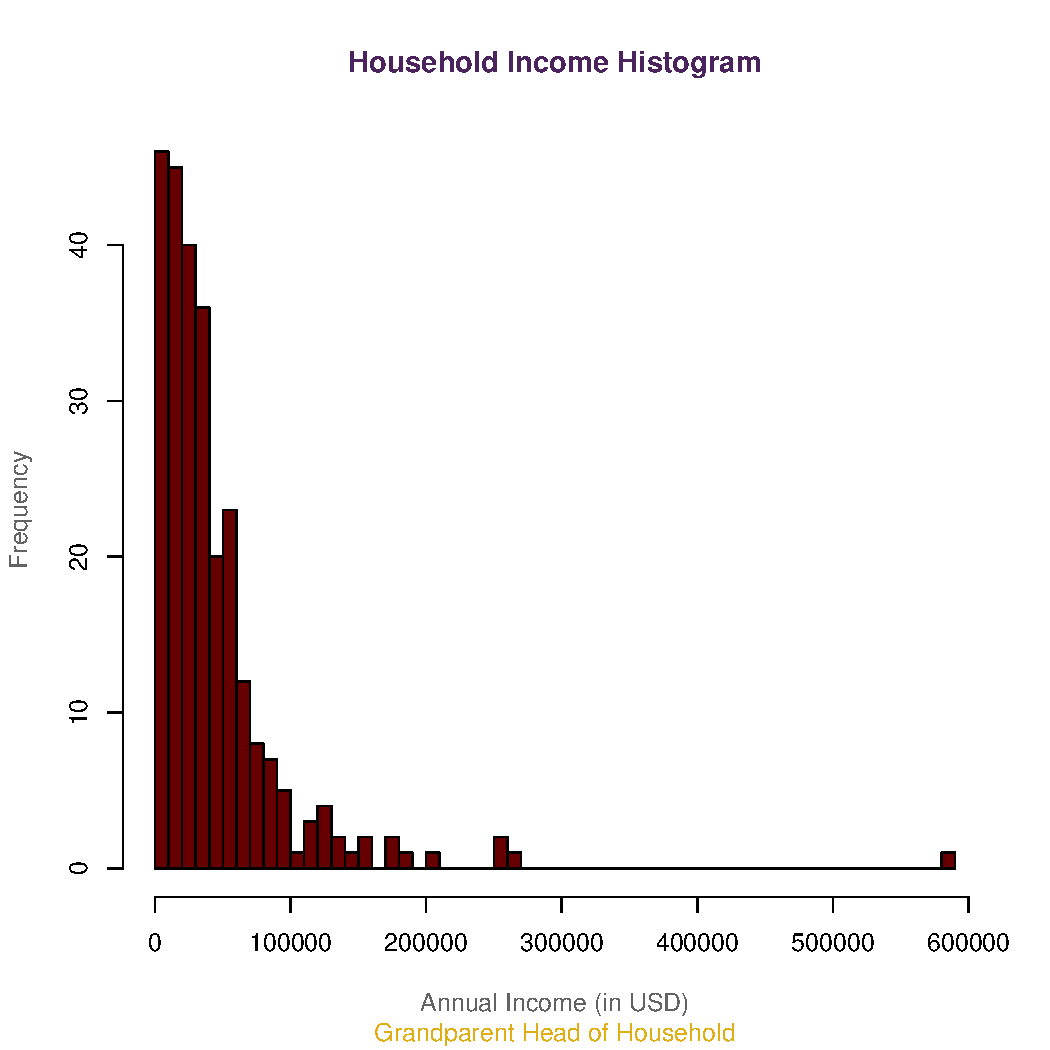
\includegraphics[width = .5\linewidth]{hist_ghh}
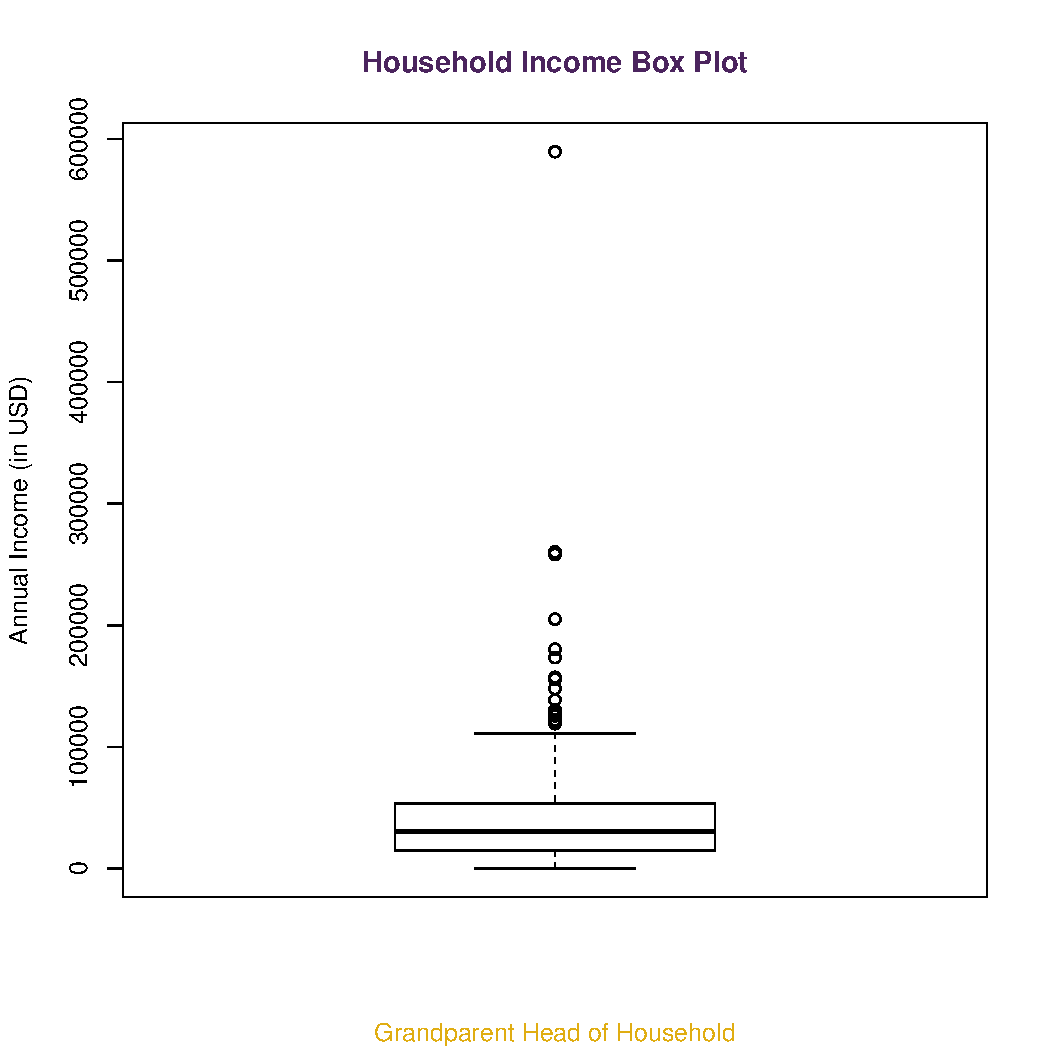
\includegraphics[width = .5\linewidth]{box_ghh}

\newpage
\appendix
\section{Source Code}

The following code can be run using \verb|source("acs_pums_analysis.R")| from R. This source code downloads the raw data file from the source.

\verbatiminput{../acs_pums_analysis.R}

\end{document}